\section{Constrained rigid body dynamics\label{constraints}}

\subsection{Approaches to constraints}
The methods developed so far allow the simulation of a single rigid body with forces
acting on it. Further challenges arise when we consider multibody systems in which the bodies
interact in some way. We will primarily be interested in articulated bodies, that is, systems
of individual rigid bodies held together by joints. Joints allow rotation but cannot be
separated.

There are various strategies for simulating articulated bodies:

\begin{itemize}
\item \emph{Penalty methods} conceptually join bodies together with springs so that when they
    begin to separate, a restoring force causes them to move back together again. These methods
    are simple to implement initially but hard to get right: if the springs are too weak, the
    bodies will separate too far; if they are too stiff, very large forces can arise suddenly,
    causing the simulation to become unstable. Penalty methods only become active after the
    system has already entered an illegal state, which may be undesirable.

\item Mechanics formulations using \emph{generalized coordinates} build constraints firmly into
    the system: the number of generalized coordinates equals the actual number of degrees of
    freedom after the constraints have been applied. The state of the system is specified only in
    terms of these generalized coordinates, and they are chosen such that the system will always
    be in a legal state, irrespective of what the values of the coordinates are. Outside
    influences can be transformed into the generalized coordinates. The most famous formulation
    along these lines is \emph{Lagrangian mechanics}~\cite{Hand:98,Goldstein:80} which is
    commonly used in physics, but alternatives are described in~\cite{Wilhelms:91}
    and~\cite{Featherstone:87}.
    These algorithms have in common that they allow very fast and reliable computation. However,
    the functions to transform the coordinates must be determined analytically, and this becomes
    very hard or impossible for complicated systems, so the method does not scale or generalize
    well. And even if the equations can be solved, these methods are limited to so-called
    \emph{holonomic constraints} (see~\cite{Hand:98} for a definition). Joints, for example,
    are holonomic, while separable contact points between bodies are not.

\item A compromise between the flexibility of penalty methods and the stability of generalized
    coordinates can be found. As in the penalty method, we initially treat each limb of an
    articulated body separately and grant it its full six degrees of freedom. We then impose
    constraints on the system which prevent the limbs from separating or moving in other
    undesirable ways. Crucially, we formulate the constraints in such a way that we can not only
    tell whether the system is currently in an illegal state, but also whether it is moving
    towards one, and even whether it is accelerating towards one. Using the method of
    \emph{Lagrange multipliers} we can determine what forces must be applied to the bodies to
    nullify this unwanted acceleration before it ever occurs. This compromise comes at the expense
    of higher computational cost, because systems of linear equations have to be solved at
    run-time. Note that despite the similarity in name, this method has very little in common with
    Lagrangian mechanics.
\end{itemize}

I chose to use Lagrange multiplier constraints to implement articulated body dynamics in this
project, because the algorithm is very general-purpose and can, for example, be adapted to handle
some types of non-holonomic constraint.
The mathematical formulation of Lagrange multipliers is derived in~\cite{BaraffWitkin:97} and
extended in~\cite{Saunders:PhD} (also see~\cite{Baraff:96} for an optimized algorithm),
therefore I shall only state the results here.

\subsection{Prerequisites of constraint solving}

Consider a system of $n$ rigid bodies at a particular point in time. Assume that we can define
a vector \ve{x} which represents the state of the whole system as a function of
time\footnote{Witkin~\cite{BaraffWitkin:97} calls this vector \ve{q}; I use \ve{x} to avoid
confusion with quaternions.}. \ve{x} has $6n$ rows (one row for each d.o.f.)\ and its first and
second derivative with respect to time are
\begin{equation}
\label{lagrangeStateVector}
\dot{\ve{x}} = \left[ \begin{array}{c}
    \dot{\ve{r}}_1\\ \ve{\omega}_1\\ \vdots\\ \dot{\ve{r}}_n\\ \ve{\omega}_n \end{array}\right]
\quad\quad\mathrm{and}\quad\quad
\ddot{\ve{x}} = \left[ \begin{array}{c}
    \ddot{\ve{r}}_1\\ \dot{\ve{\omega}}_1\\ \vdots\\ \ddot{\ve{r}}_n\\ \dot{\ve{\omega}}_n
    \end{array}\right]
\end{equation}
where $\ve{r}_i$ is the position of the centre of mass of body $i$, and $\ve{\omega}_i$ is its
angular velocity. Thus $\dot{\ve{x}}$ is the concatenation of all bodies' linear and angular
velocities, and $\ddot{\ve{x}}$ is that of the accelerations. We cannot write down an explicit
expression for \ve{x} since we do not have a representation of orientation whose derivative is
\ve{\omega}! This is not a problem though, since we can work exclusively with $\dot{\ve{x}}$ and
$\ddot{\ve{x}}$.

We require two more vectors in the same format, containing the forces and torques already acting
on the system, for example due to gravity or muscular activity:
\begin{equation} \label{PhiVector}
\ve{\Phi} = \left[\begin{array}{c}
    \ve{F}_1 \\ \ve{\tau}_1 \\ \vdots \\ \ve{F}_n \\ \ve{\tau}_n
    \end{array}\right]
    \quad\quad\quad
\ve{\Phi}_p = \left[\begin{array}{c}
    \ve{0} \\ -\dual{\ve{\omega}_1}\m{I}_1\ve{\omega}_1 \\ \vdots \\
    \ve{0} \\ -\dual{\ve{\omega}_n}\m{I}_n\ve{\omega}_n
    \end{array}\right]
\end{equation}

Here $\ve{F}_i$ denotes the sum of all forces acting on the centre of mass of body~$i$, and
$\ve{\tau}_i$ is the sum of all torque vectors acting on body~$i$. The vector $\ve{\Phi}_p$
accounts for the fact that a body's moment of inertia is in general not constant in the world
frame\footnote{The subscript $p$ of this vector stands for \emph{precession}, since the
variability of the moment of inertia causes free precession.}; $\m{I}_i$ is body $i$'s moment
of inertia in the world frame at the current point in time.
See appendix~\ref{correctBrettAppendix} for a derivation of $\ve{\Phi}_p$.

Following the same principle of concatenation, we set up the inverse mass-inertia matrix
$\m{M}^{-1}$, a $6n\times6n$ matrix of the form
\begin{equation}
\label{massInertiaTensor}
\m{M}^{-1} = \left[ \begin{array}{ccccccc}
    \frac{1}{\mu_1}\m{1} \\ & \m{I}_1^{-1} \\ &&
    \frac{1}{\mu_2}\m{1} \\ &&& \m{I}_2^{-1} \\ &&&& \ddots \\ &&&&&
    \frac{1}{\mu_n}\m{1} \\ &&&&&& \m{I}_n^{-1}
    \end{array}\right]
\end{equation}

$\mu_i$ denotes the (scalar) mass of body $i$, \m{1} stands for the $3\times3$
identity matrix, and $\m{I}_i^{-1}$ is the inverse of the inertia tensor (written as a
$3\times3$ matrix) of body $i$ in the world frame. All empty regions are zero. While $\mu_i$
will typically stay constant over time, $\m{I}_i$ may depend on the orientation of body
$i$.\footnote{If we know the principal axes of the body, we can express \m{I} in a time-invariant
form combined with rotations into the principal axes frame and back again
(see~\cite{BaraffWitkin:97}), which saves us a lot of effort.} These variables have been chosen
such that
\begin{equation}
\ddot{\ve{x}} = \m{M}^{-1} (\ve{\Phi} + \ve{\Phi}_p).
\end{equation}

\subsection{Lagrange multipliers}

Now assume that we want to impose $m$ constraints on this system, where each constraint
effectively reduces the number of degrees of freedom by one. Express each constraint as a function
$c$ which is zero when the constraint is satisfied. (A ball-and-socket joint, which allows three
modes of rotation but no separation, reduces the number of d.o.f.\ by three and is therefore
expressed as a vector of three scalar constraint functions.) We can then concatenate all
constraint functions into a single $m$-row constraint vector \ve{c}. Each valid configuration of
the system must satisfy $\ve{c} = \ve{0}$, the null vector.

To find the constraint maintaining forces, we must know how a change in state or a change in
time affects the value of \ve{c}. To this end, we must calculate the first two derivatives of
\ve{c} with respect to time, $\dot{\ve{c}}$ and $\ddot{\ve{c}}$. We also calculate the Jacobian
matrix~\cite{RHB:02} \m{J} which contains all partial derivatives of $\ve{c}$ w.r.t.\ each
coordinate of \ve{x}, and the similarly defined Jacobian $\dot{\m{J}}$ of $\dot{\ve{c}}$:
\begin{equation}
J_{ij} = \frac{\partial c_i}{\partial x_j} \quad\quad\mathrm{and}\quad\quad
\dot{J}_{ij} = \frac{\partial \dot{c}_i}{\partial x_j}
\end{equation}

Both $\m{J}$ and $\dot{\m{J}}$ are $m \times 6n$ matrices. However, since we do not
have an explicit expression for \ve{x}, we cannot calculate them directly using
partial differentiation. Instead we make use of the following analytic results:
\begin{equation}
\label{cDotAndCDDot}
\dot{\ve{c}} = \m{J}\dot{\ve{x}} \quad\quad\mathrm{and}\quad\quad
\ddot{\ve{c}} = \dot{\m{J}}\dot{\ve{x}} + \m{J}\ddot{\ve{x}}.
\end{equation}

Any Jacobian component $J_{ij}$ is certainly zero if constraint $i$ does not mention body
$\lfloor j/6 \rfloor$. Since constraints are usually only between two bodies, \m{J} and
$\dot{\m{J}}$ each have a sparse block-structured form sketched in figure~\ref{jacobianFigure}.
If there are many constraints, their slices of the Jacobian can be calculated independently and
simply inserted at the right places in \m{J} and $\dot{\m{J}}$. Appendix~\ref{constraintAppendix}
gives derivations of Jacobian slices for different constraint types.

\begin{figure}
\psfrag{frag:1}{$1$}
\psfrag{frag:i}{$i$}
\psfrag{frag:j}{$j$}
\psfrag{frag:m}{$m$}
\psfrag{frag:6n}{$6n$}
\psfrag{frag:jac}{$\m{J}=\left(\rule{54mm}{0mm}\rule{0mm}{20mm}\right)$}
\psfrag{frag:b1}{$\begin{array}{c} b_1 \\ \overbrace{\rule{0mm}{5mm}} \end{array}$}
\psfrag{frag:b2}{$\begin{array}{c} b_2 \\ \overbrace{\rule{0mm}{5mm}} \end{array}$}
\psfrag{frag:ci}{$\ve{c}_i$}
\centerline{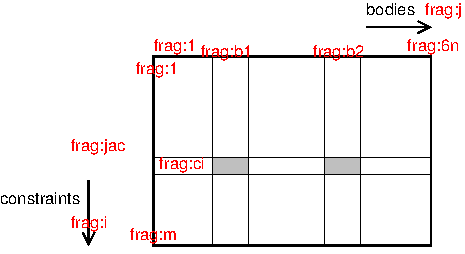
\includegraphics{figures/jacobian}}
\caption[]{Block structure of the Jacobian matrix of $m$ constraints in a system of $n$ bodies.
    For example, if $\ve{c}_i$ is a ball-and-socket joint between bodies $b_1$ and $b_2$, each of
    the two slices is three rows high and six columns wide. The vertical position of $\ve{c}_i$
    must match its offset in the concatenated constraint vector \hbox{\ve{c}}, and the horizontal
    positions must match the offset of bodies $b_1$ and $b_2$ in the vectors $\dot{\ve{x}}$,
    \ve{\Phi} and $\ve{\Phi}_p$ (equations~\ref{lagrangeStateVector} and~\ref{PhiVector}).
    \label{jacobianFigure}}
\end{figure}

Now that all is prepared, we can set up the equation\footnote{Here we adopt the sign convention
of~\cite{BaraffWitkin:97}, which is the opposite of~\cite{Saunders:PhD}.}
\begin{equation}
\label{lagrangeEquation}
-\m{J}\m{M}^{-1}\m{J}^T\ve{\lambda} = \dot{\m{J}}\dot{\ve{x}} +
    \m{J}\m{M}^{-1}(\ve{\Phi} + \ve{\Phi}_p) + k\ve{c} + d\dot{\ve{c}}
\end{equation}
in which all variables except $\ve{\lambda}$ are known. The meaning of this equation and
its two scalar constants $k$ and $d$ is discussed in~\cite{BaraffWitkin:97}
and~\cite{Saunders:PhD}. For us it will suffice to consider it to be a `black box' which can be
given to a linear equation solver to obtain $\ve{\lambda}$.

$\ve{\lambda}$ is an $m$-row vector of so-called \emph{Lagrange multipliers} (after which this
algorithm is named), where $m$ is the number of constraints. Once we have solved for it, we can
compute the expression
\begin{equation} \label{lagrangeSolution}
\ve{\Phi}_c = \m{J}^T\,\ve{\lambda}.
\end{equation}
$\ve{\Phi}_c$ has the same format as $\ve{\Phi}$, and indeed it is the vector containing
the forces and torques which we need to additionally apply to each body to ensure that they
continue to satisfy the constraints! All we therefore need to do is to compute
$\ve{\Phi} + \ve{\Phi}_c$ and to feed the result into our ODE solver. $\ve{\Phi}_p$ must not
be added to this term if the moment of inertia is recalculated based on the bodies' orientation.
